\renewcommand{\theequation}{\theenumi}
%\subsection{Problem}

\begin{enumerate}[label=\arabic*.,ref=\thesection.\theenumi]
\numberwithin{equation}{enumi}

\item
The following python script plots 
%
\begin{align}
f(\lambda) = a\lambda^2 + b\lambda + d
\label{eq:parab}
\end{align}
%
for 
\begin{align}
a &= \norm{\vec{m}}^2 > 0
\\
b &= \vec{m}^T\brak{\vec{A} -\vec{P}} 
\\
c &= \norm{\vec{A} -\vec{P}}^2
\end{align}
where $\vec{A}$ is the intercept of the line $L$ in \eqref{eq:opt_line_nor}
on the x-axis and the points
\begin{align}
\vec{U} &= \myvec{\lambda_1\\f(\lambda_1)}, 
\vec{V} = \myvec{\lambda_2\\f(\lambda_2)}
\\
\vec{X} &= \myvec{t \lambda_1 + \brak{1-t}\lambda_2 \\ f\sbrak{t \lambda_1 + \brak{1-t}\lambda_2}},
\\
\vec{Y} &= \myvec{t \lambda_1 + \brak{1-t}\lambda_2 \\ t f\brak{\lambda_1} + \brak{1-t}f\brak{\lambda_2}}
\end{align}
%
for 
\begin{align}
\lambda_1 = -3, 
\lambda_2 = 4, 
t = 0.3
\end{align}
in Fig. \ref{fig:conv_def}. Geometrically, this means that any point $\vec{Y}$ between the points $\vec{U}, \vec{V}$ on the line $UV$ is always above the point $\vec{X}$ on the curve $f(\lambda)$.
Such a  function $f$ is defined to be {\em convex} function 
%
\begin{lstlisting}
codes/optimization/1.2.py
\end{lstlisting}
%
%%
\begin{figure}[!ht]
\centering
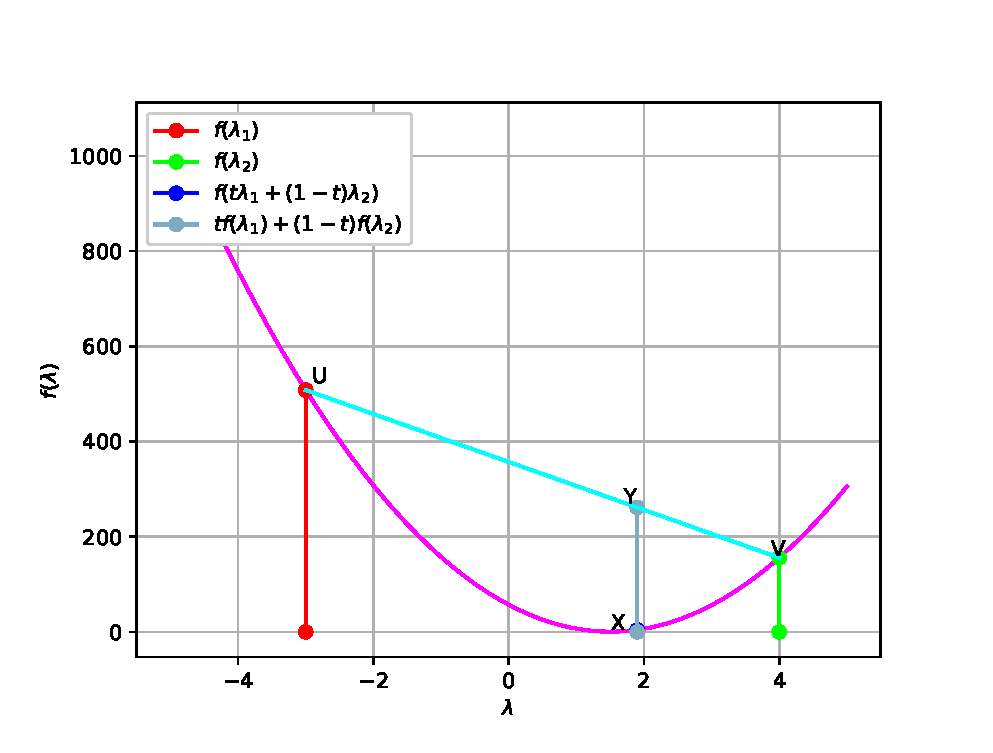
\includegraphics[width=\columnwidth]{./figs/convex.eps}
\caption{ $f(\lambda)$ versus $\lambda$}.
\label{fig:conv_def}	
\end{figure}
%
\item Show that
%
\begin{align}
\label{eq:convex_def}
f\sbrak{t \lambda_1 + \brak{1-t}\lambda_2} \leq 
t f\brak{\lambda_1} + \brak{1-t}f\brak{\lambda_2}
\end{align}
%
for $\quad 0 < t < 1$.  This is true for any convex function.\\
%
\textbf{Solution: } Consider a convex function $f$. By the definition of a convex function, a secant joining any two points on $f$ should lie above the graph $y=f(x)$.\\
Consider the two points to be $(\lambda_1,f(\lambda_1))$ and $(\lambda_2,f(\lambda_2))$ and a value $t$ such that $0 < t < 1$.\\
A point on the secant between those points will be \\ 
$(t\lambda_1+(1-t)\lambda_2,t f(\lambda_1)+(1-t)f(\lambda_2))$ \\
The point on the $y=f(x)$ at corresponding x coordinate will be\\ 
$(t\lambda_1+(1-t)\lambda_2, f\sbrak{t\lambda_1+(1-t)\lambda_2})$\\
For the secant to lie above the graph, y-coordinate of point on secant should be above the y-coordinate of corresponding point on the graph.\\
i.e $ f\sbrak{t\lambda_1+(1-t)\lambda_2} \leq f(\lambda_1)+(1-t)f(\lambda_2)$

\item Show that 
%
\begin{equation}
\eqref{eq:convex_def} \quad \implies f^{(2)}(\lambda) > 0
\end{equation}
%
\textbf{Solution: }Consider three points $(a,f(a)),$ $(b,f(b))$ and $(c,f(C))$ such that $a<b<c$.\\
\eqref{eq:convex_def} with $t=\frac{c-b}{c-a}$ and $\lambda_1 =a$, $\lambda_2 =c$ gives
\begin{center}
    $f(b) \leq \sbrak{\frac{c-b}{c-a}}f(a) + \sbrak{\frac{b-a}{c-a}}f(c)$
\end{center}
%
which solves to for any $a<b<c$,
\begin{align}
    \frac{f(b)-f(a)}{b-a} \leq \frac{f(c)-f(a)}{c-a}
\end{align}
%
Apply limits
\begin{align*}
    \lim_{b-a\to 0}\frac{f(b)-f(a)}{b-a} &\leq \lim_{c-b\to 0}\frac{f(c)-f(b)}{c-b} \\
    \implies f^{(1)}(b) \leq f^{(1)}(c)\\
    \implies f^{(1)}(c) - f^{(1)}(b) &\geq 0 
\end{align*}  

Because $c-b > 0$
\begin{align*}
    \frac{f^{(1)}(c) - f^{(1)}(b)}{c-b} &\geq 0
\end{align*}  
%
Apply limit
\begin{align*}  
    \lim_{c-b\to 0} \frac{f^{(1)}(c) - f^{(1)}(b)}{c-b} & \geq 0\\
    \implies f^{(2)}(c) & \geq 0 \numberthis 
\end{align*} 
%
As a,b,c are chosen arbitrarily with $a<b<c$ for any $\lambda$ in domain of f,\\
\begin{align}
{f^{(2)}(\lambda) \geq 0}
\end{align}
%
%
%
\item Show that a convex function has a unique minimum.\\
%
\textbf{Solution:}
Consider a convex function $f$ having global minimum at $x_1$ and local minimum at $x_2$ ($x_1\neq x_2$)
\begin{center}
    i.e $f(x_1)\leq f(x_2)$
\end{center}
From the definition of convexity, we have for $0< \theta<1$,
\begin{center}
    $f(\theta x_1+(1 - \theta)x_2) \leq \theta f(x_1)+(1 - \theta)f(x_2) $
\end{center}
Since $\theta$ is positive
\begin{equation} 
\begin{split}
    f(x_1)\leq f(x_2)\implies\theta f(x_1)\leq \theta f(x_2)
\end{split}
\end{equation}
which justifies below condition
\begin{equation} \label{eq1}
\begin{split}
    \theta f(x_1)+(1-\theta)f(x_2) &\leq \theta f(x_2)+(1-\theta)f(x_2)\\
    &\leq f(x_2)
\end{split}
\end{equation}
Replacing this condition to the definition of convexity
\begin{center}
    $f(\theta x_1+(1-\theta)x_2) \leq f(x_2)$
\end{center}
If $x_2$ is a local minimum, the neighborhood must be defined such as $f(x)\geq f(x_2)$.\\
To satisfy both conditions it must be that 
\begin{center}
    $f(x) = f(x_1) = f(x_2) \forall x_1\leq x\leq x_2 $
\end{center}
which shows that f has a unique minimum value.
%
\end{enumerate}
%
